\def\year{2019}\relax
%File: formatting-instruction.tex
\documentclass[letterpaper]{article} %DO NOT CHANGE THIS
\usepackage{aaai19}  %Required
\usepackage{times}  %Required
\usepackage{helvet}  %Required
\usepackage{courier}  %Required
\usepackage{url}  %Required
\usepackage{graphicx}  %Required
\usepackage{amssymb}
\usepackage{amsmath}
\usepackage[sort&compress,square,comma,authoryear]{natbib}

\usepackage{amsfonts}
\usepackage{amssymb}
\usepackage{amsthm}
\usepackage{bbm}
\usepackage{latexsym}
\usepackage{mathtools}
\usepackage{color}

\usepackage{algorithm}
\usepackage{algorithmic}


\frenchspacing  %Required
\setlength{\pdfpagewidth}{8.5in}  %Required
\setlength{\pdfpageheight}{11in}  %Required


%PDF Info Is Required:
  \pdfinfo{
/Title (2019 Formatting Instructions for Authors Using LaTeX)
/Author (AAAI Press Staff)}
\setcounter{secnumdepth}{0}  

\DeclareMathOperator*{\argmin}{argmin}
\DeclareMathOperator*{\argmax}{argmax}

\newcommand{\km}[1]{{\color{red} #1}} %red comments: Karsten
\newcommand{\wb}[1]{{\color{blue} #1}} %blue comments: Walter

\begin{document}
% The file aaai.sty is the style file for AAAI Press 
% proceedings, working notes, and technical reports.
%
\title{Facility Location Utility for Uncovering Unknown Unknowns}
\author{Karsten Maurer$^1$ \hspace{.2in} Walter Bennette$^2$\\
$^1$Miami University Department of Statistics - maurerkt@miamioh.edu\\ 
$^2$Air Force Research Lab Information Directorate - walter.bennette.1@us.af.mil \\
}

\maketitle
\begin{abstract}
AAAI creates proceedings, working notes, and technical reports directly from electronic source furnished by the authors. To ensure that all papers in the publication have a uniform appearance, authors must adhere to the following instructions. 
\end{abstract}

\section{Introduction}

Techniques such as active learning \citep{Settles2010} and domain adaptation \citep{Patel2014} can be used to create machine learning classifiers when large labeled datasets are not available for a specific task.  For example, the black box classifiers made available through many online services (list services) require no training data and can be thought of as a kind of domain adaptation.  However, with limited amounts of labeled data, users may not be able to properly evaluate a model, and are left hoping the model will be useful for their intended task.  In this paper we build upon previous work to develop an interactive method to help evaluate classifiers in the absence of labeled data.  Specifically, we develop an interactive method to uncover unknown unknowns \citep{Attenberg2015}: instances for which a classifier is confident in its prediction, but is wrong.  

Intuitive methods can be used to evaluate the performance of a model in the absence of labeled data.  Given a labeling budget one could sample instances following an experimental design, sample instances with the lowest classifier confidence, or sample instances identified as informative to the classifier through active learning strategies.  These methods could provide a sense of a model's performance but will potentially miss high confidence mistakes, referred to as \textit{unknown unknowns}.     

Unknown unknowns can be thought of as blind spots to a classification model, and can be caused by dataset bias during training, domain shift during use, lack of model expressibility, and other causes of poor model fit.  From the viewpoint of a rational actor, unknown unknowns represent costly mistakes because minimal risk mitigation strategies will have been deployed for these high confidence predictions.  The discovery of unknown unknowns may allow new mitigation strategies to be formulated \citep{Nushi2016a}.  Additionally, as enumerated in \citep{Bansal2018}, finding unknown unknowns is valuable to understand classifier limitations and prevent attacks (stole this hard) \km{what do you mean by attacks?}

\citet{Attenberg2015} gamified the search for unknown unknowns and relied on human oracles to discover misclassified instances. A utility-based search algorithm for discovering unknown unknowns was then proposed by \citet{Lakkaraju2016} and expanded upon by \citet{Bansal2018}. \citet{Lakkaraju2016} uses a utility model that simply counts the number of discovered unknown unknowns and searches using multi-armed bandits. \citet{Bansal2018} argued that this unit utility model motivates the discovery of very similar unknown unknowns. To fix this problem they proposed an adaptive coverage-based utility model that attempts to encourage the discovery of unknown unknowns throughout the feature space, favoring high confidence regions. They then search for unknown unknowns via a greedy algorithm to maximize utility. 

The utility in \citet{Bansal2018} has the form: $$U(Q) = \sum_{x \in \mathbb{X}} c_x \cdot \max_{q \in S} \left\{sim\left(x,q \right) \right\}$$ where $\mathbb{X} \subset \mathbb{R}^p$ is the set of available $p$-dimensional unlabeled test instances, $Q \subset \mathbb{X}$ is the set of instances labeled by an oracle, $S = \left\{x|x \in Q, y_x \neq M(x)\right\}$ is the set of discovered unknowns unknowns for some classifier $M(x):\mathbb{X} \rightarrow class$, $c_x$ is the classifier's confidence in its prediction of $x$, and $sim(x,q)$ is a distance based similarity metric.  The instance $q'$ that maximizes the expected utility increase is greedily selected to be labeled by the oracle $$E\left[U_x\left(Q \cup q'\right)\right] = \hat{\phi}(x) \cdot c_x \cdot \max_{q \in S \cup q'} \left\{sim\left(x,q \right) \right\}$$ where $\hat{\phi}(x) = P\left(y_x \neq M(x) |Q \right)$ is a conditional probability that $x$ is misclassified given the query set.  As previously stated, this method is designed to incentivize a broader search for unknown unknowns and gives higher utility for finding misclassifications in higher confidence regions.  

Unfortunately, the method of \citet{Bansal2018} is consistently outperformed by sequentially querying the instances for which the classifier is most uncertain, as shown in Figure \cite{something}.  We believe this exposes a flaw in the coverage-based utility model.  That is, the coverage-based utility model rewards the discovery of misclassified instances in close proximity to instances for which the classifier has high confidence.  This reward strategy would help find high confidence unknown unknowns if instances with similar model prediction confidence scores were near each other in the feature space, but this does not seem to be the case.

\begin{figure}[hbtp]
  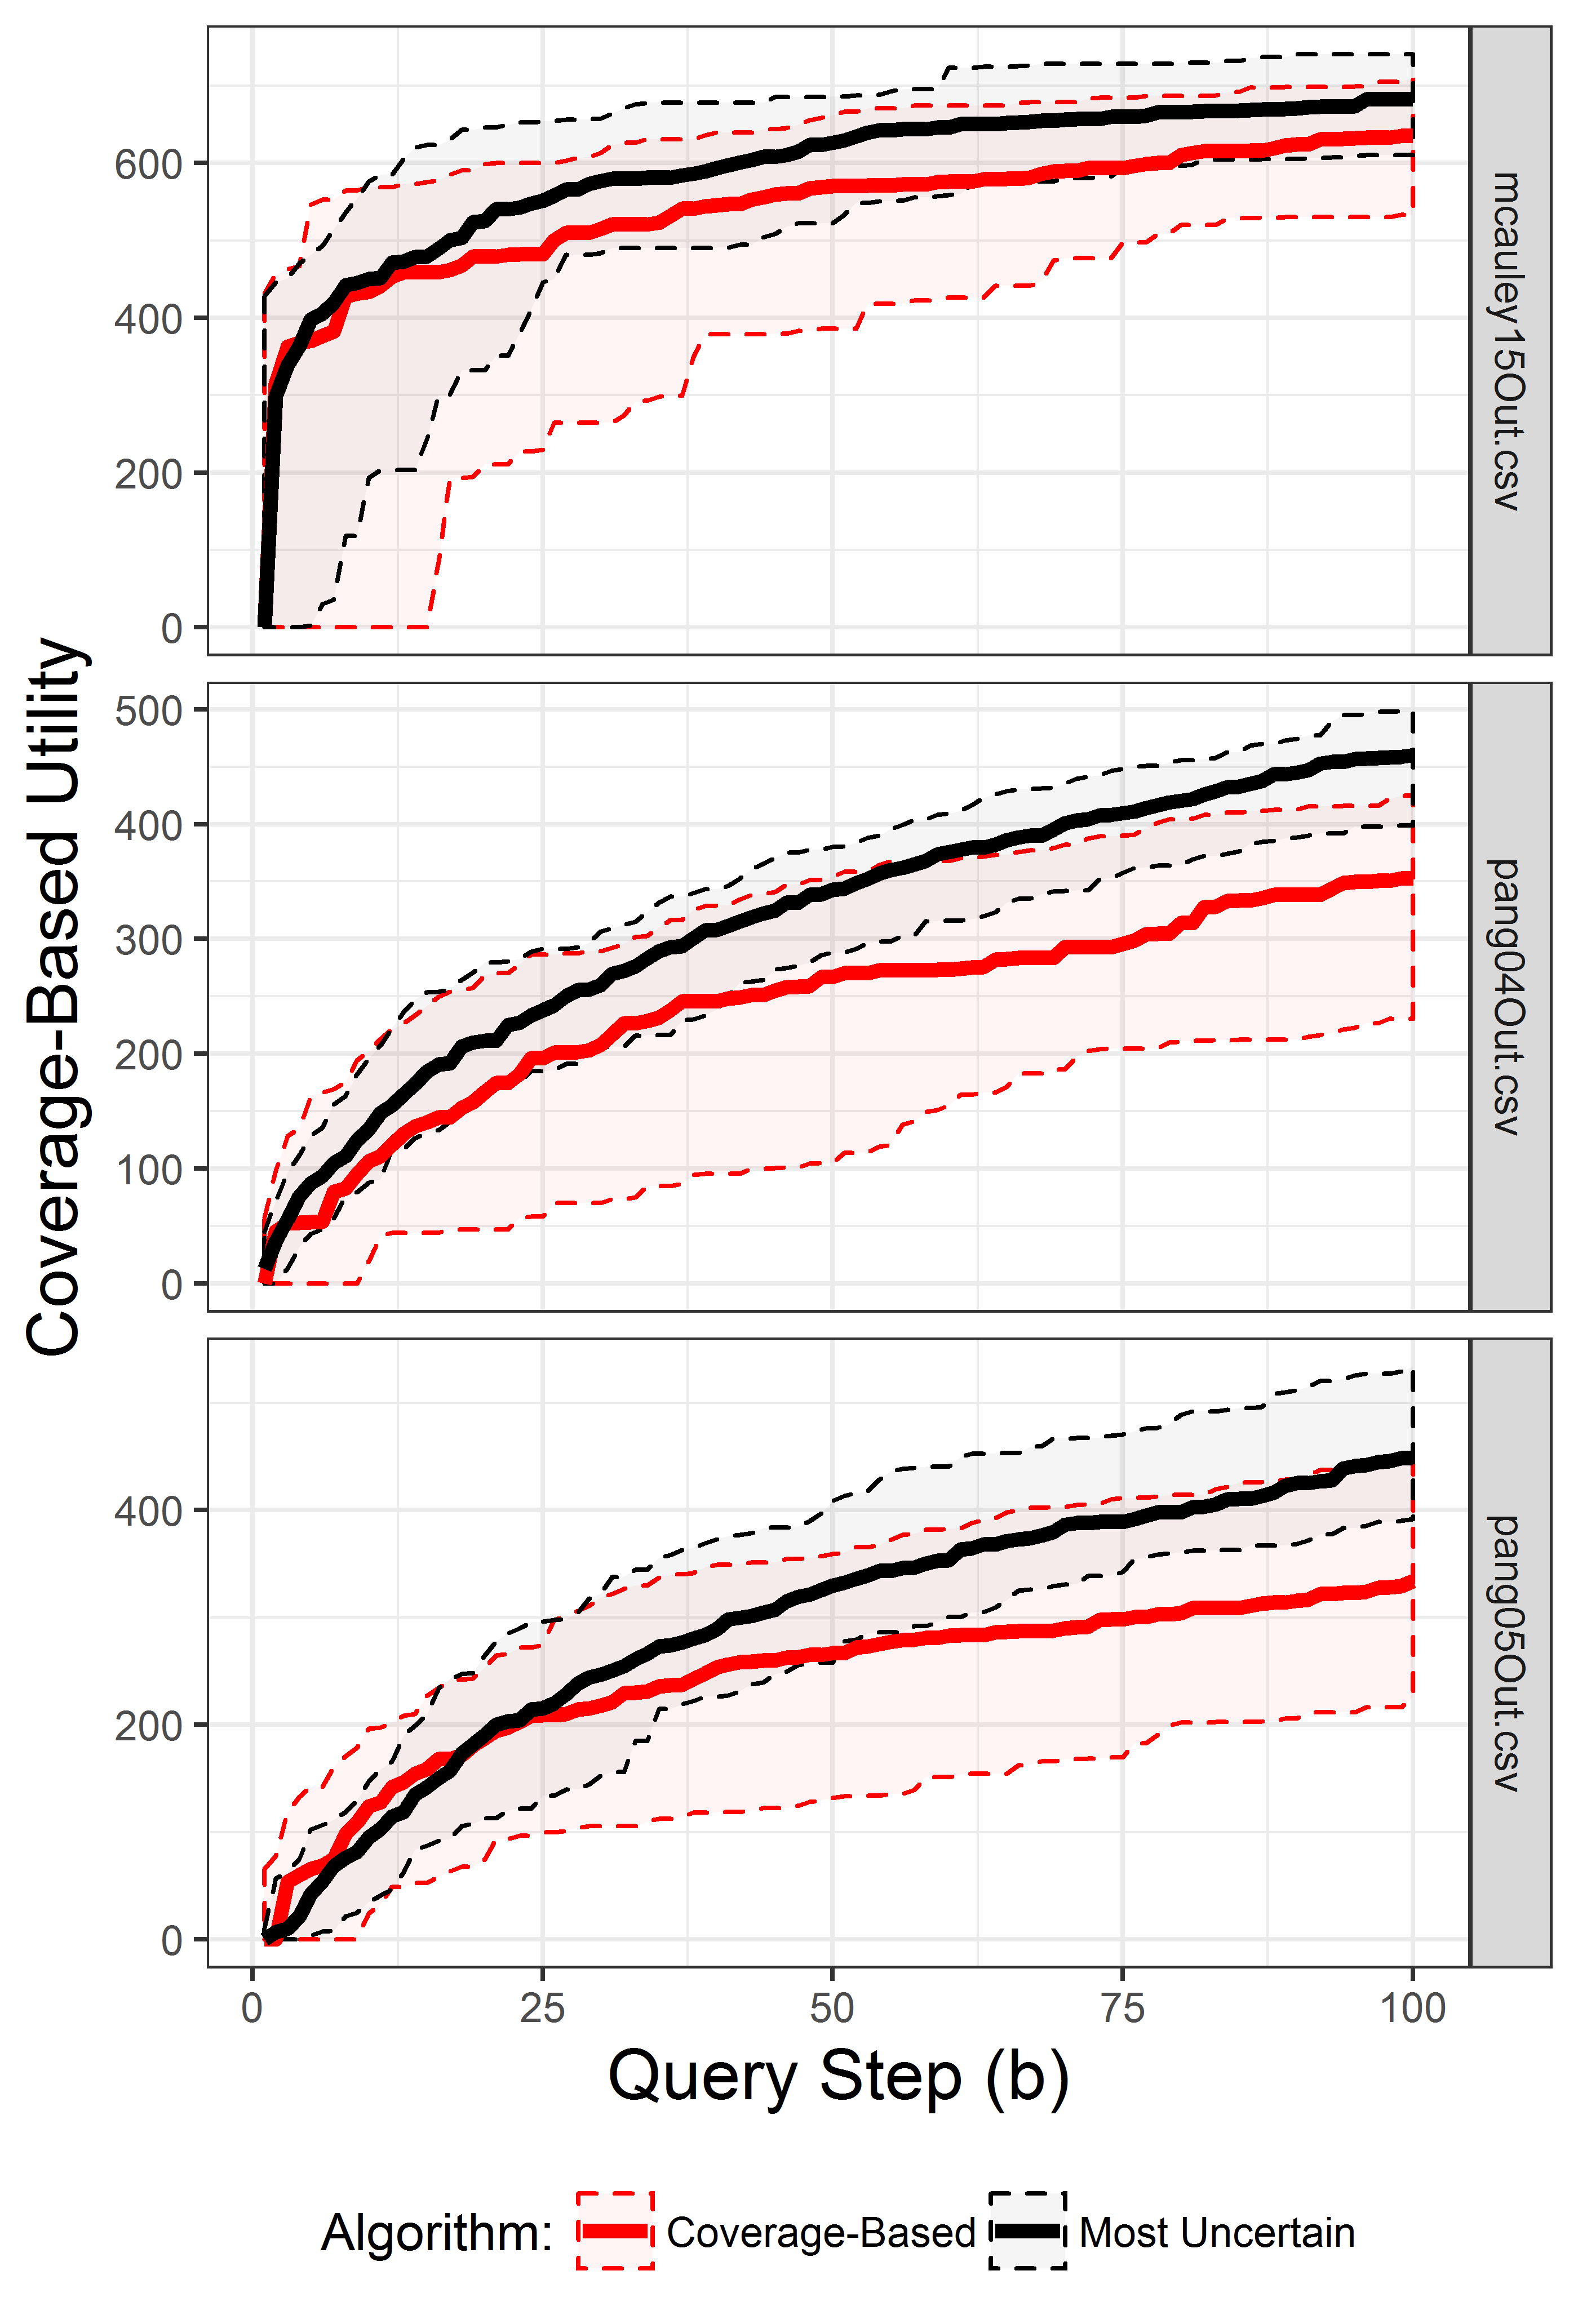
\includegraphics[width=.45\textwidth]{../experimentsAndPlots/CoverageVsMostUncertainPlaceholder.png}
  \caption{Empirical evidence that Coverage-Based Utility reward low confidence search.}
  \label{fig:coverutil}
\end{figure}



What we find wrong...

\section{Problem Formulation}


\section{Methodology}

We propose an alternative utility model based roughly on facility location optimization methods  \km{(Farahani and Hekmatfar, 2009)}. In the facility location problem a utility can be constructed that uses a greedy algorithm to minimize the cost, or maximize the reward, of building a series of new facilities in a supply chain, while also minimizing distances between clients to the nearest facility  \km{(Guha and Khuller, 1999; Arya et al., 2004)}. In the UU query setting, we can draw an analog to the selection of a point to query to the establishment of a facility at that location in the feature space; evaluating the reward for selecting the point, and the distance it stands from the surrounding unobserved points. We propose a facility location utility function as: 

$$W(Q) = \sum_{x \in S} r \left(c_x\right) - \frac{1}{n} \sum_{x \in \mathbb{X}} \min_{q \in S}\left(d\left(x,q\right)\right)$$

where $r\left(c_x\right) = \log($1/$(1-c_x))$ is the reward function for finding an UU with confidence $c_{x}$, and $d(x,q)$ is the Euclidean distance between points $x$ and $q$. We use the greedy algorithm that at each iteration selects $q'$ with the maximum expected utility, as defined in Algorithm 1 below. 

%	FISTA with separation
\begin{algorithm}
	\caption{Greedy Facility Location Search}
	\label{alg:Greedy}
	\begin{algorithmic}
		\STATE {\bfseries Input:} Test set $\mathbb{X}$, prior $\hat{\phi}\left(x|Q=\emptyset\right)$, budget B
		\STATE $Q=\{\}$ \{inputs that have been queried\}
		\STATE $y_Q = \{\}$ \{oracle defined labels\}
		\STATE{\bfseries For: } $b = 1, 2, ..., B$ {\bfseries do:}

		\STATE $q' = \argmax_{q' \not\in Q} E \left[W\left(Q \cup q'\right) \right]$
		
		\STATE $y_{q'} = OracleQuery(q')$
		\STATE $Q \leftarrow Q \cup q'$
		\STATE $S \leftarrow \left\{x | x \in Q \space \text{ and } y_x \neq M(x) \right\}$
		\STATE $b \leftarrow b + 1$
			

		\STATE {\bfseries Return: $Q$ and $y_q$}
	\end{algorithmic}
\end{algorithm}

At each iterative step in Algorithm 1, we need to select the point that will maximize the expected gain in facility location utility, given probability estimates for point misclassification, such that  $\hat{\phi}(q' | Q) = \hat{P}(y_{q'} \ne M(q' ) |  Q )$. To find the expected gain in utility for each point, we evaluate the utility under the possibilities that the point is either misclassified or correctly classified. These possible utility outcomes are then averaged with weights equal to the estimated probability of each outcome. Thus the optimization step requires the solution of the following:

$$\underset{q' \notin Q}{argmax} E[W(Q \cup q')] = $$
\begin{equation*}
\small
\underset{q' \notin Q}{argmax} \left[\begin{split}
\hat{\phi}(q') \cdot \left[\sum_{x \in S \cup q'} r \left(c_x\right) - \frac{1}{n} \sum_{x \in \mathbb{X}} \min_{q \in S \cup q'}\left(d\left(x,q\right)\right) \right] + \\ 
(1-\hat{\phi}(q')) \cdot \left[\sum_{x \in S} r \left(c_x\right) - \frac{1}{n} \sum_{x \in \mathbb{X}} \min_{q \in S}\left(d\left(x,q\right)\right)\right]  
\end{split}\right]
\end{equation*}
\normalsize

Note that $\left[\sum_{x \in S} r \left(c_x\right) - \frac{1}{n} \sum_{x \in \mathbb{X}} \min_{q \in S}\left(d\left(x,q\right)\right)\right]$ is constant for all considered points, but cannot simply be removed from the argmax solution because it is multiplied by an estimated probability that is unique to each point. 

There are several characteristics to note in the design of the facility locations utility model. First, the rewards are only accumulated by finding UUs in the query set, this avoids the issue of placing value on points in the test set for simply having high confidence points; whereas having a small average minimum distance between all test points to their closest observed UU is also seen as valuable for encouraging strong coverage by the query set. 

The reward function is designed to impact the utility in a way that is consistent with a limiting factor being the budget for oracle queries. Viewed as a geometric distribution problem with a probability $\phi(x)$ of discovering a UU, we expect to need 1/$\phi(x)$ queried points before discovering the first UU \km{(Casella and Berger, 2002)}. For heuristic insight into the reward behavior construction, if we assume that   $\phi(x) ~= (1-c_x )$, then our reward is a log-scaled count of the number of randomly selected points we would expect to query in order to find the UUs in our query set. The higher this number becomes, the more efficient our search was. We use the log scaling to avoid over-incentivizing the search for incredibly rare UUs, as we know there is a limited budget for oracle queries. While seemingly convoluted, it avoids an important pitfall of summing the confidences directly, where we would inherently incentivize the most-uncertain search pattern by default. As an example, suppose we have a budget of ten oracle queries: if we select all points with $(1-c_x )=0.7$ then we might expect to find three UUs – thus gain a reward of 2.1; as opposed to when $(1-c_x )=0.9$ then we expect to find only one – thus gain a reward of 0.9. Under the proposed reward function for this example, we expect an equal reward for finding the expected number of UUs given their confidence: $3\cdot r(.7)=1\cdot r(.9)=10$. The optimization step will provide the highest expected reward for selecting the most overconfident point relative to the updated probability estimates, that is to say when %(1-c_Mx )<< \hat{\phi}(x)$. Note that unlike the UU definition, this construction does not depend on the arbitrary definition of a confidence threshold, τ, beyond which we search for misclassifications. The reward component of the facility locations utility should encourage the query set to select any points where the model is most overconfident.

In addition to a change to the utility structure, we have explored the use of alternative model-based estimates for $\hat{\phi}(x)$. In this paper we demonstrate the use of logistic regression classifiers as alternatives to the cluster-based probabilities used in  \textbf{Bansal and Weld’s (2018)} adaptive greedy algorithm.  


\section{Experimental Evaluation}

\begin{figure}[hbtp]
  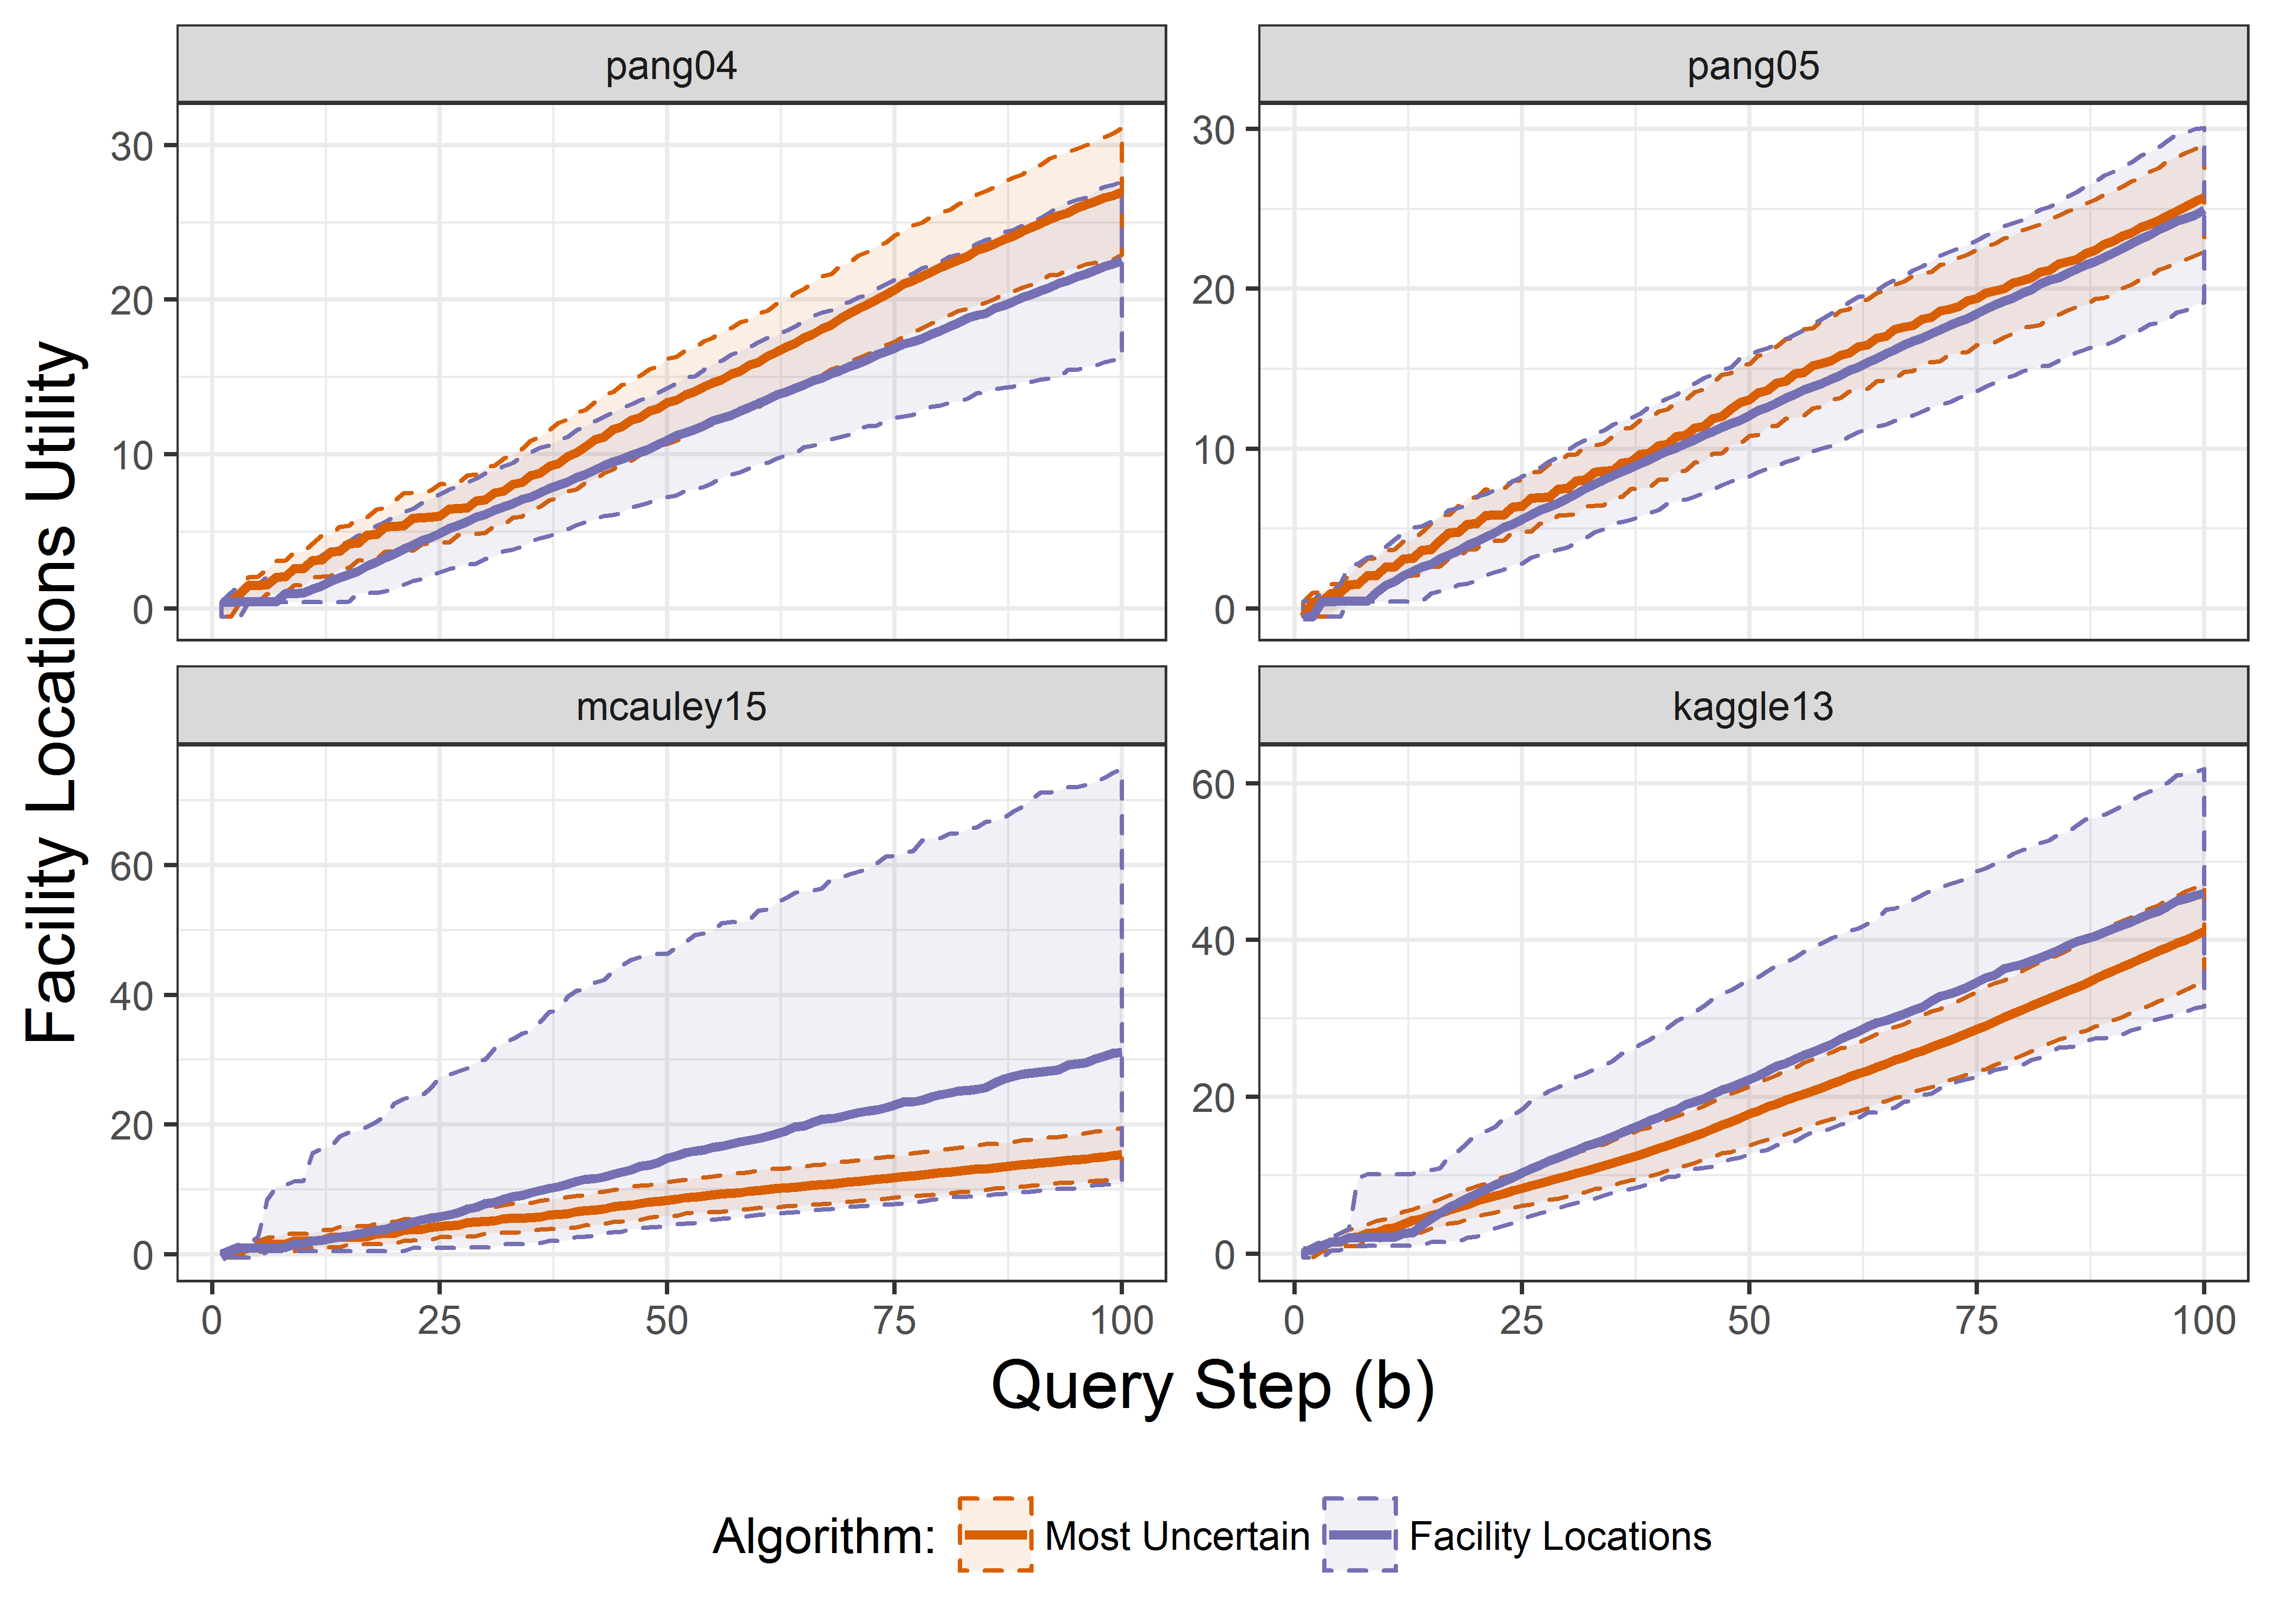
\includegraphics[width=.45\textwidth]{../experimentsAndPlots/flUtilPlaceholder.png}
  \caption{Faciltiy Locations Utility rewards finding overconfidence.}
  \label{fig:coverutil}
\end{figure}


\section{Discussion \& Conclusions}



\newpage
\bibliographystyle{aaai}

\bibliography{library}


\end{document}
